\documentclass{customDoc}
\usepackage{colortbl}
\usepackage{booktabs}
\usepackage{gensymb}
\usepackage{longtable}
\usepackage{multirow}
\usepackage{graphicx}
\usepackage{subcaption}
\usepackage[per-mode=symbol]{siunitx}
\sisetup{detect-all}
\usepackage{multicol}
\usepackage{float}
\usepackage[inkscapelatex=false]{svg}
\usepackage{pstricks}

\begin{document}
\title{同轴电缆实验 - 实验报告}
\class{トレセン学園 高等部二年生}
\name{アドマイヤベガ}
\id{1}
\maketitle

\section{摘要}

本实验主要探究同轴电缆的电容和电感,以及传输特性,并通过实验测量同轴电缆的电容和电感值,分析其传输特性. 实验中使用了示波器、信号发生器等仪器,测量并计算了同轴电缆的特性阻抗和传输损耗.

\section{实验原理}

同轴电缆可以视为圆柱形的电感或电容,同时对应一个 $LC$ 等效电路,可以计算其传输性质. 长度为 $l$,内外半径分别为 $a$ 和 $b$ 的同轴电缆,其电容和电感分别为:

\begin{equation}
    C = \frac{2\pi\varepsilon_0l}{\ln(b/a)} \quad L = \frac{\mu_0l}{2\pi}\ln(b/a)
\end{equation}

由此也可以计算单位长度的电容和电感. 当电磁波经同轴电缆传播时,可以定义同轴电缆的传播常数 $\gamma$ 和特征阻抗 $Z_0$:

\begin{equation}
    \gamma = \sqrt{(R+\text{j}\omega L)(G+\text{j}\omega C)}\,,\quad Z_0 = \sqrt{\frac{R+\text{j}\omega L}{G + \text{j}\omega C}}
\end{equation}

其中 $R$ 和 $G$ 分别为单位长度的电阻和导纳. 在实验中,我们可以通过测量入射 (出射) 波电压和入射 (出射) 波电流之比来计算特征阻抗.

\section{实验仪器及实验步骤}

(1) 信号发生器 (泰克 AFG1062,双通道,\SI{60}{M\hertz},采样率 \SI{300}{MS/s});

(2) 示波器(罗德施瓦茨 RTM3004,四通道,\SI{100}{M\hertz},采样率 \SI{5}{GS/s});

(3) 测试线,约 \SI{1}{m} 长,两端均为 SMA 阳头 (SMA 是 SubMiniature version A 的缩写. SMA 接头是一种应用广泛的小型螺纹连接的同轴连接器),共 4 根,已接在信号发生器和示波器上;

(4) \SI{1}{\kilo\ohm} 电阻,电阻盒侧面贴有“$R=\SI{1}{\kilo\ohm}$”标签;

(5) \SI{10}{\ohm} 电阻,电阻盒侧面贴有“$R=\SI{10}{\ohm}$”标签. 电阻也接在同轴电缆中心导体上;

(6) \SI{50}{\ohm} 电阻负载,电阻接在同轴接头内外导体之间;

(7) 短路负载,将同轴接头的内外导体短路;

(8) 三通接头若干,每个接头有 3 个相互连通的 SMA 阴头;

(9) 同轴电缆,共使用 4 根 \SI{4.8}{\metre} 长的 SMA 接头同轴电缆.

实验步骤如下:

1. 测量同轴电缆的等效电容和电感;

2. 计算特征阻抗和传播速度;

3. 探究电磁波在同轴电缆不同负载下的传输与反射;

4. 探究简谐信号在同轴电缆中的驻波.

\section{数据处理}

\subsection{测量同轴电缆的等效电容和电感}

测量数据如下:

% Table generated by Excel2LaTeX from sheet 'Sheet1'
\begin{table}[htbp]
  \centering
  \caption{测量同轴电缆的等效电容和电感}
    \begin{tabular}{|r|c|l|r|c|l|}
    \hline
    \multicolumn{3}{|c|}{电容} & \multicolumn{3}{c|}{电感} \\
    \hline
    CH1 频率 & 69.9877 & \si{\kilo\hertz}   & CH1 频率 & 270.031 & \si{\kilo\hertz} \\
    \hline
    CH1 峰峰值 & 20.286 & \si{\volt}     & CH1 峰峰值 & 5.18  & \si{\volt} \\
    \hline
    CH2 峰峰值 & 15.141 & \si{\volt}     & CH2 峰峰值 & 3.2346 & \si{\volt} \\
    \hline
    $V_R$ 峰峰值 & 14.307 & \si{\volt}     & $V_R$ 峰峰值 & 3.4961 & \si{\volt} \\
    \hline
    相位差   & -89.95 & \si{\degree}     & 相位差   & 78.59 & \si{\degree} \\
    \hline
    \end{tabular}
\end{table}

计算电容和电感:

\begin{equation}
    \begin{aligned}
    C_1 &= \frac{V_R}{2\pi fV_{CH1}R} = \SI{2.14878E-09}{\farad} \Longrightarrow C = \frac{C_1}{l} = \SI{1.11916E-10}{\farad/\metre} \\
    L_1 &= \frac{RV_{CH1}}{2\pi fV_R} = \SI{5.4531E-06}{\henry} \Longrightarrow L = \frac{L_1}{l} = \SI{2.84015E-07}{\henry/\metre}
    \end{aligned}
\end{equation}

\subsection{计算特征阻抗和传播速度}

用上面已经测得的数据计算特征阻抗:

\begin{equation}
    Z_0 = \sqrt{\frac{L}{C}} = \SI{50.37620034}{\ohm}
\end{equation}

同时可以计算电磁波在同轴电缆中传播的相速度和介质的相对介电常数:

\begin{equation}
    v_p = \frac{1}{\sqrt{LC}} = \SI{177371318.1}{\metre/\second} \quad \epsilon_r = \frac{c^2}{v_p^2} = 2.856765675
\end{equation}

\subsection{探究电磁波在同轴电缆不同负载下的传输与反射}

界面处的电压反射系数:

\begin{equation}
    \Gamma = \frac{V_r}{V_i} = \frac{Z_1 - Z_0}{Z_1 + Z_0}
\end{equation}

理论上,当 $Z_1 = Z_0$ 时,没有反射,这被称为阻抗匹配条件. 同时当 $Z_1 = 0$ 时,反射系数为 $-1$,相位变化为 $\pi$ (反相).

测量开路状态下的同轴电缆的信号幅度 $V_i$ 和信号延时 $\tau_i$,数据如下:

% Table generated by Excel2LaTeX from sheet 'Sheet1'
\begin{table}[htbp]
  \centering
  \caption{开路状态信号数据}
    \begin{tabular}{|c|c|c|}
    \hline
    序号    & $V_i$ (\si{\milli\volt}) & $\tau_i$ (\si{\nano\second}) \\
    \hline
    0     & 480.44 & 102 \\
    \hline
    1     & 886.66 & 108 \\
    \hline
    2     & 792.92 & 110 \\
    \hline
    3     & 705.03 & 110 \\
    \hline
    4     & 632.77 & 108 \\
    \hline
    5     & 560.51 & 110 \\
    \hline
    6     & 499.97 & 110 \\
    \hline
    7     & 441.38 & 110 \\
    \hline
    8     & 396.46 & 112 \\
    \hline
    9     & 353.49 & 108 \\
    \hline
    \end{tabular}
\end{table}

示波器上的图像如图:

\begin{figure}[H]
    \centering
    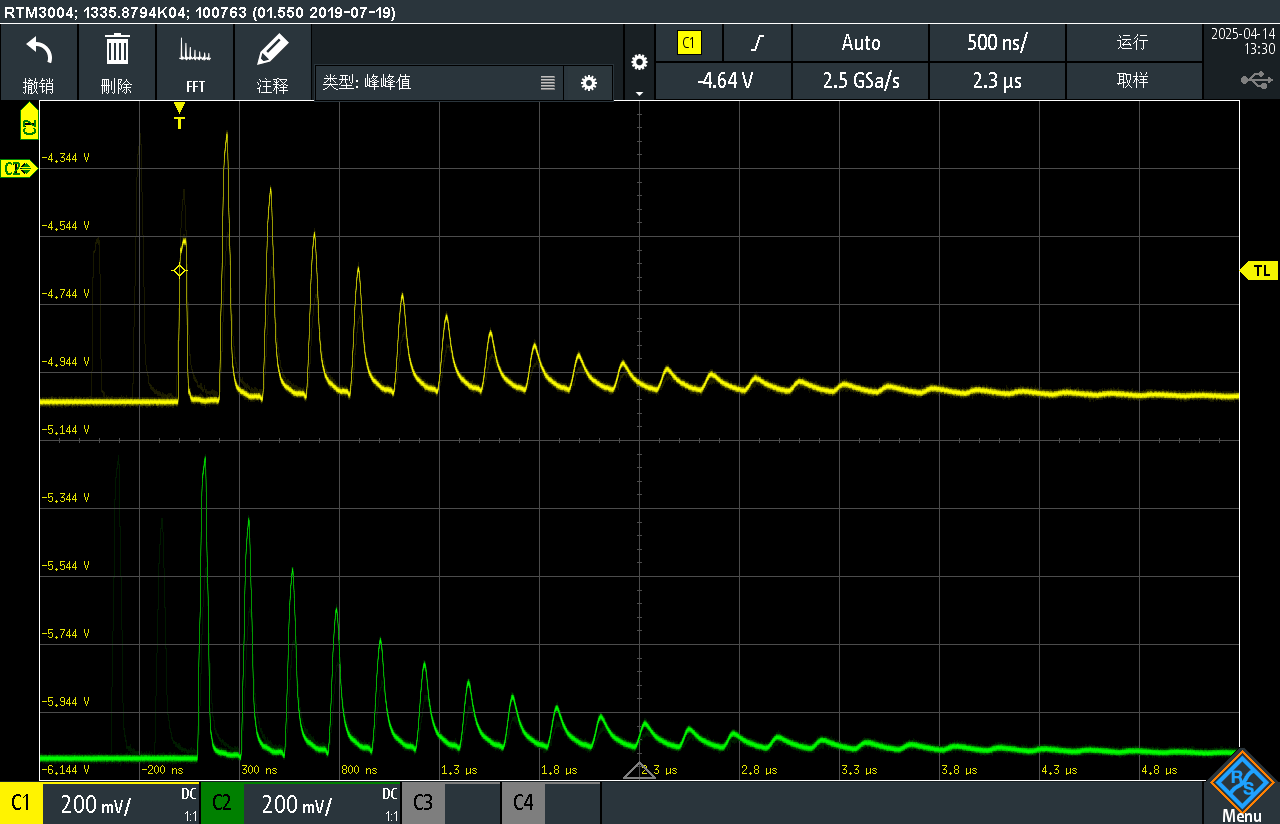
\includegraphics[width=0.8\textwidth]{SCR07.PNG}
    \caption{开路状态下的同轴电缆信号}
    \label{fig:open_circuit}
\end{figure}

拟合得到这些数据的衰减系数 $k = 0.11527$,再除以电缆长度得到同轴电缆的衰减系数:$\alpha = k / l = \SI{6.0036E-3}{\metre}^{-1}$.

解释为什么第一个信号低于后面的信号:对于 $V_0$ 的测量仅仅是入射波部分,随后的信号在始端与末端来回反射,每一个信号都测量的是入射波和反射波的和,而反射波与入射波同相叠加,因而 $V_1$ 大约是 $V_0$ 的两倍.

CH2 测试线移动到第 3 和第 4 段电缆之间,测量得到的图像如下:

\begin{figure}[H]
    \centering
    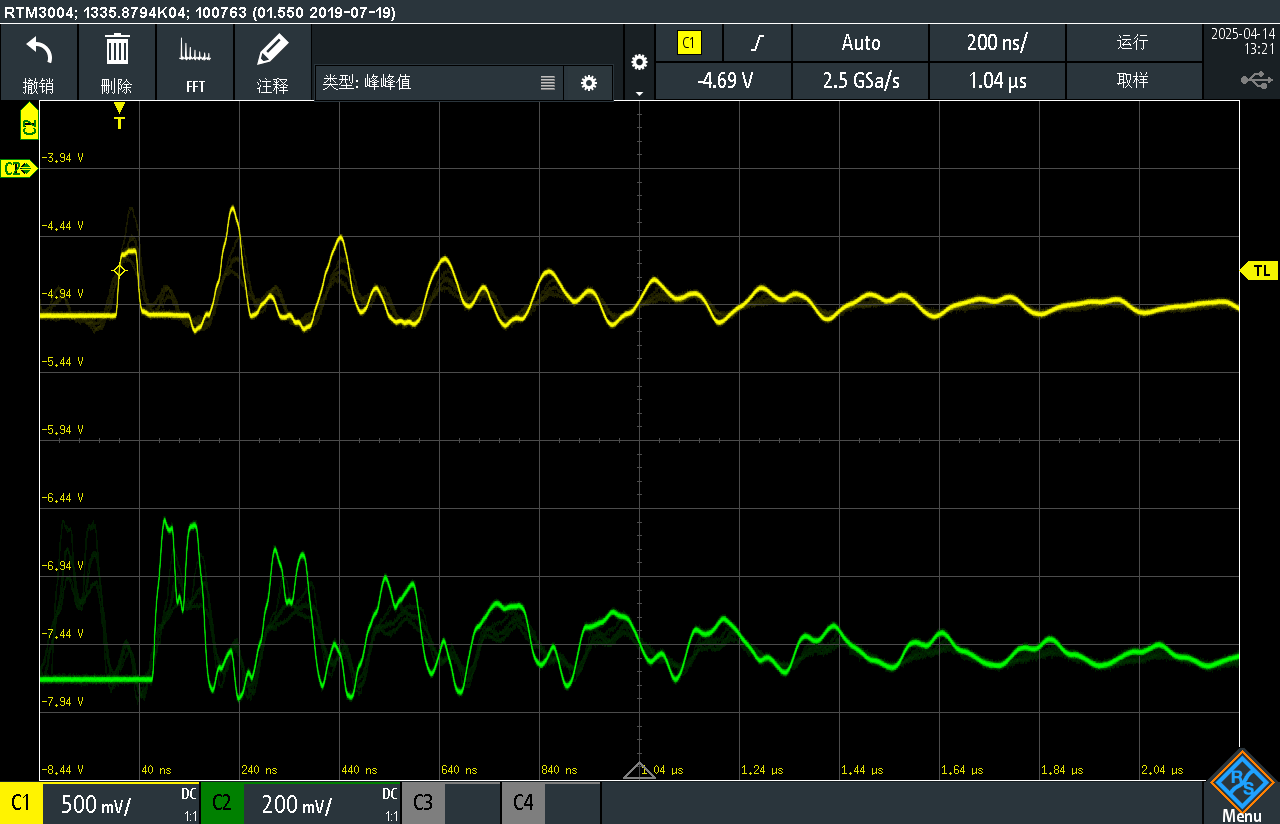
\includegraphics[width=0.8\textwidth]{SCR01.PNG}
    \caption{开路状态下的同轴电缆信号 - CH2 测试线移动}
    \label{fig:open_circuit_2}
\end{figure}

可以发现,原先的一个峰值分裂为两个峰,而且两个峰值的叠加和原来的峰值比较接近. 以最高的峰值为例,接线位置没有变化之前,为 $\SI{886.66}{\milli\volt}$,而分裂成的两个峰值分别是 $\SI{453.1}{\milli\volt}$ 和 $\SI{443.33}{\milli\volt}$,加起来为 $\SI{898.43}{\milli\volt}$,和原来的峰值的相对误差仅有 $1.3\%$,说明分裂的两个峰值在之前是同相叠加的,和我们上面的理论解释相吻合.

负载为短路时,测量得到的图像如下:

\begin{figure}[H]
\begin{subfigure}[b]{0.45\textwidth}
    \centering
    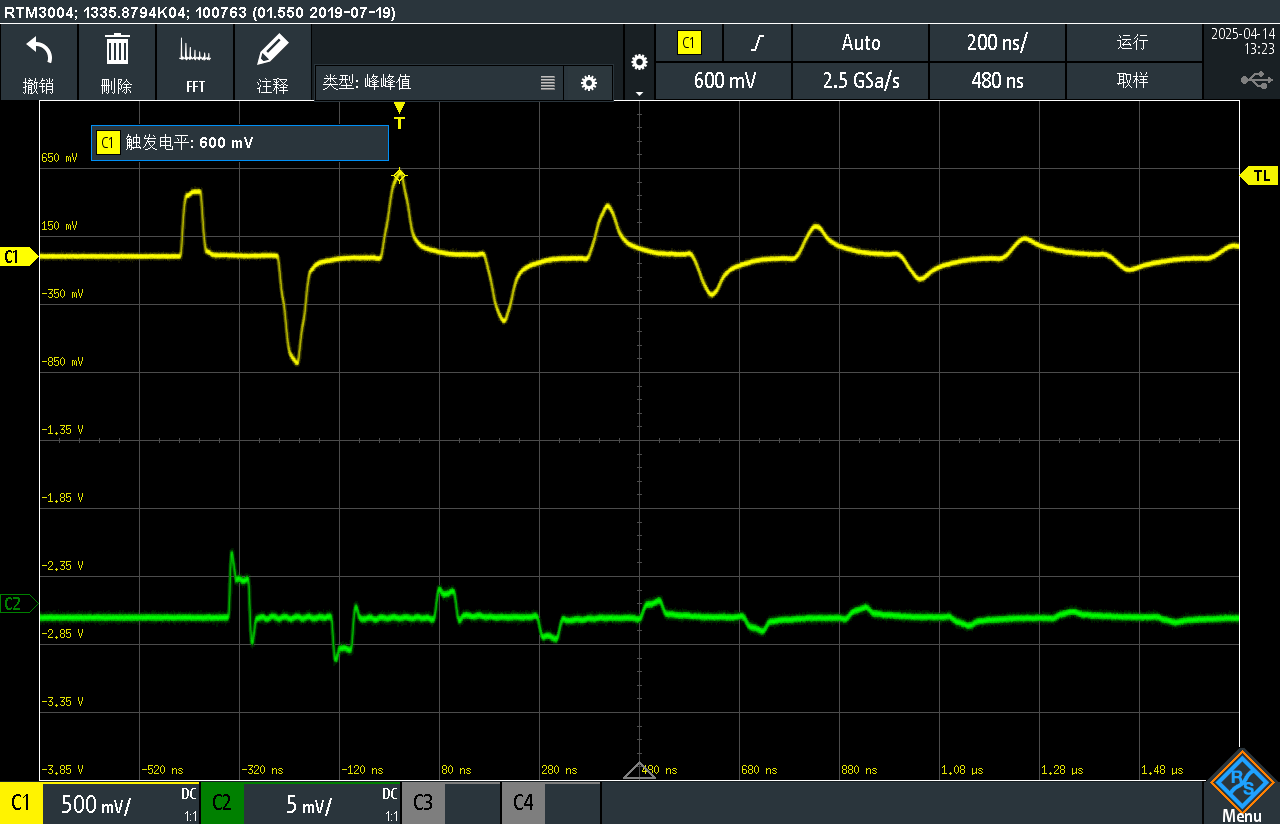
\includegraphics[width=\textwidth]{SCR02.PNG}
    \caption{CH2 测试线不移动}
    \label{fig:short_circuit_1}
\end{subfigure}
\hfill
\begin{subfigure}[b]{0.45\textwidth}
    \centering
    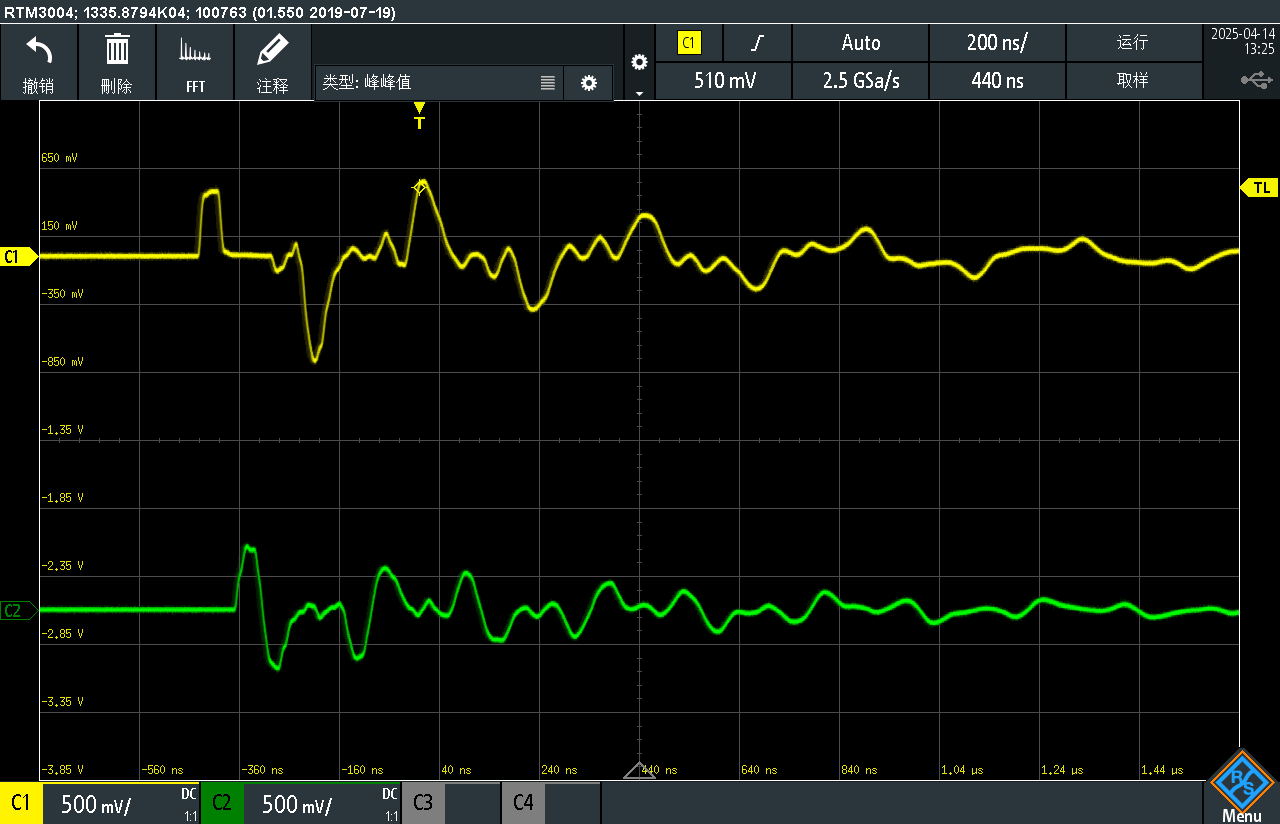
\includegraphics[width=\textwidth]{SCR03.PNG}
    \caption{CH2 测试线移动}
    \label{fig:short_circuit_2}
\end{subfigure}
\centering
\caption{短路状态下的同轴电缆信号}
\end{figure}

负载为 $\SI{50}{\ohm}$ 电阻时,测量得到的图像如下:

\begin{figure}[H]
\begin{subfigure}[b]{0.45\textwidth}
    \centering
    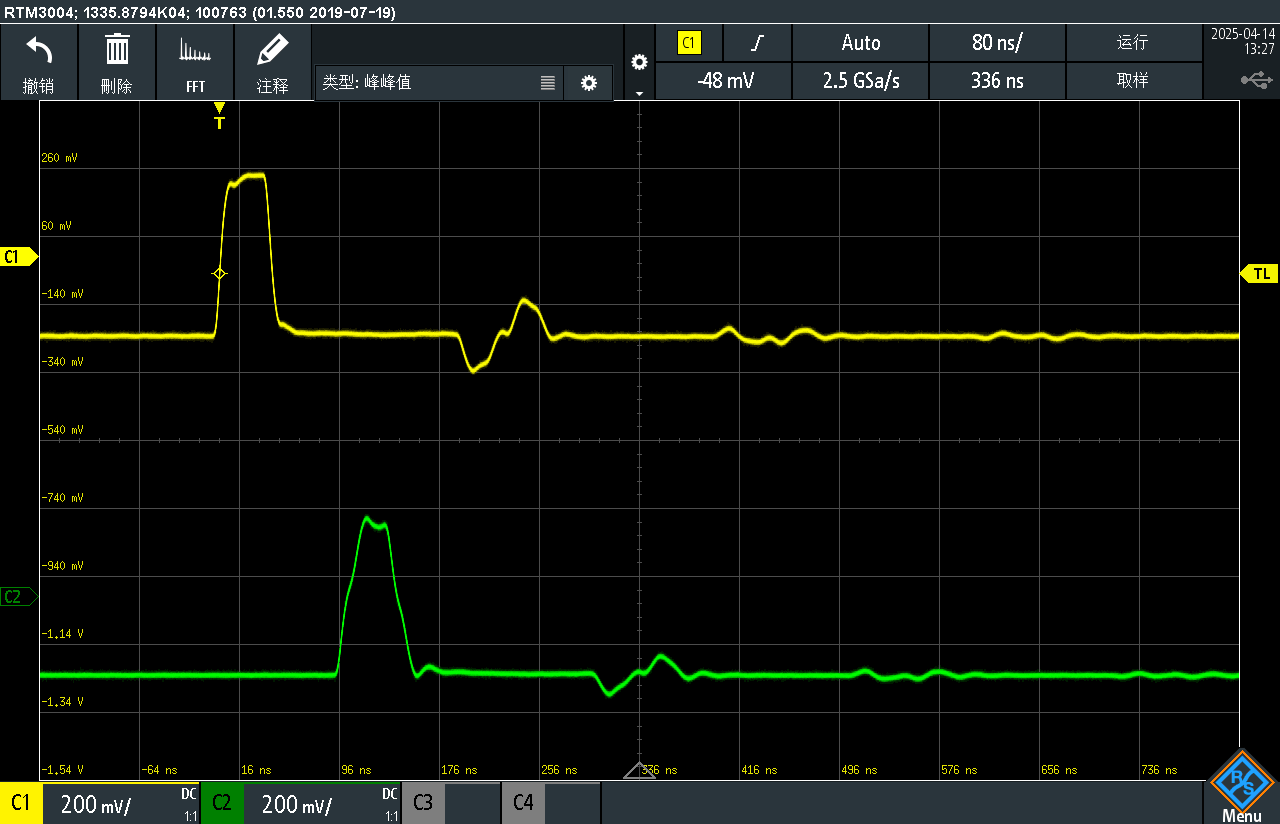
\includegraphics[width=\textwidth]{SCR05.PNG}
    \caption{CH2 测试线不移动}
    \label{fig:load_50_1}
\end{subfigure}
\hfill
\begin{subfigure}[b]{0.45\textwidth}
    \centering
    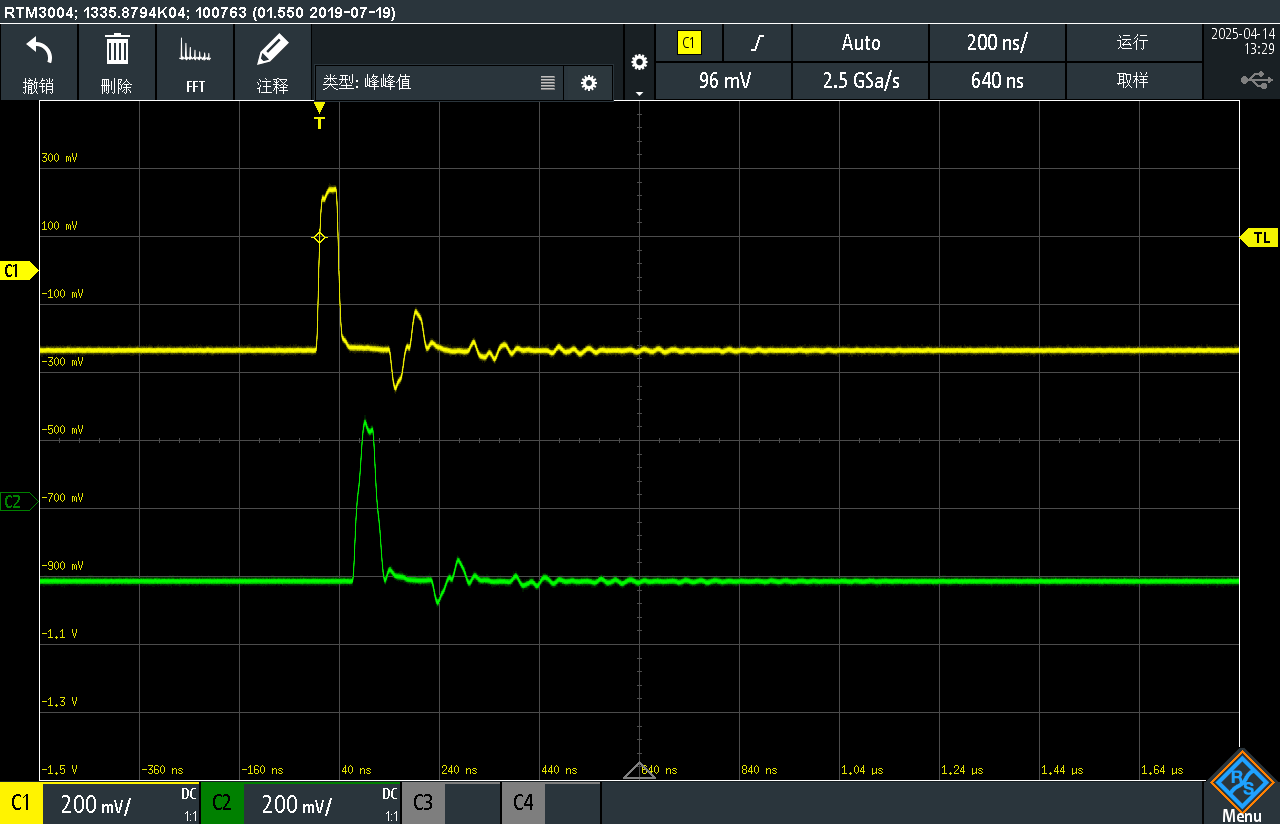
\includegraphics[width=\textwidth]{SCR06.PNG}
    \caption{CH2 测试线移动}
    \label{fig:load_50_2}
\end{subfigure}
\centering
\caption{负载为 $\SI{50}{\ohm}$ 电阻时的同轴电缆信号}
\end{figure}

\subsection{探究简谐信号在同轴电缆中的驻波}

末端开路时,反射系数为 $1$,边界条件为:

\begin{equation}
    V^+(x = 0) = V^-(x = 0) \,,\quad V^+(x = l) + V^-(x = l)
\end{equation}

因此解得驻波条件为

\begin{equation}
    f = \frac{nv_p}{2l}\,,\quad n = 1, 2, 3, \cdots\,,\quad v_p = \frac{1}{\sqrt{LC}} = \SI{177371318.1}{\metre/\second}
\end{equation}

最小的两个驻波频率是 $\SI{4619044.743}{\hertz}$ 和 $\SI{9238089.485}{\hertz}$,将信号发生器的输出频率调节为这两个值,测量得到两种情况下的图像如图所示:

\begin{figure}[H]
    \centering
    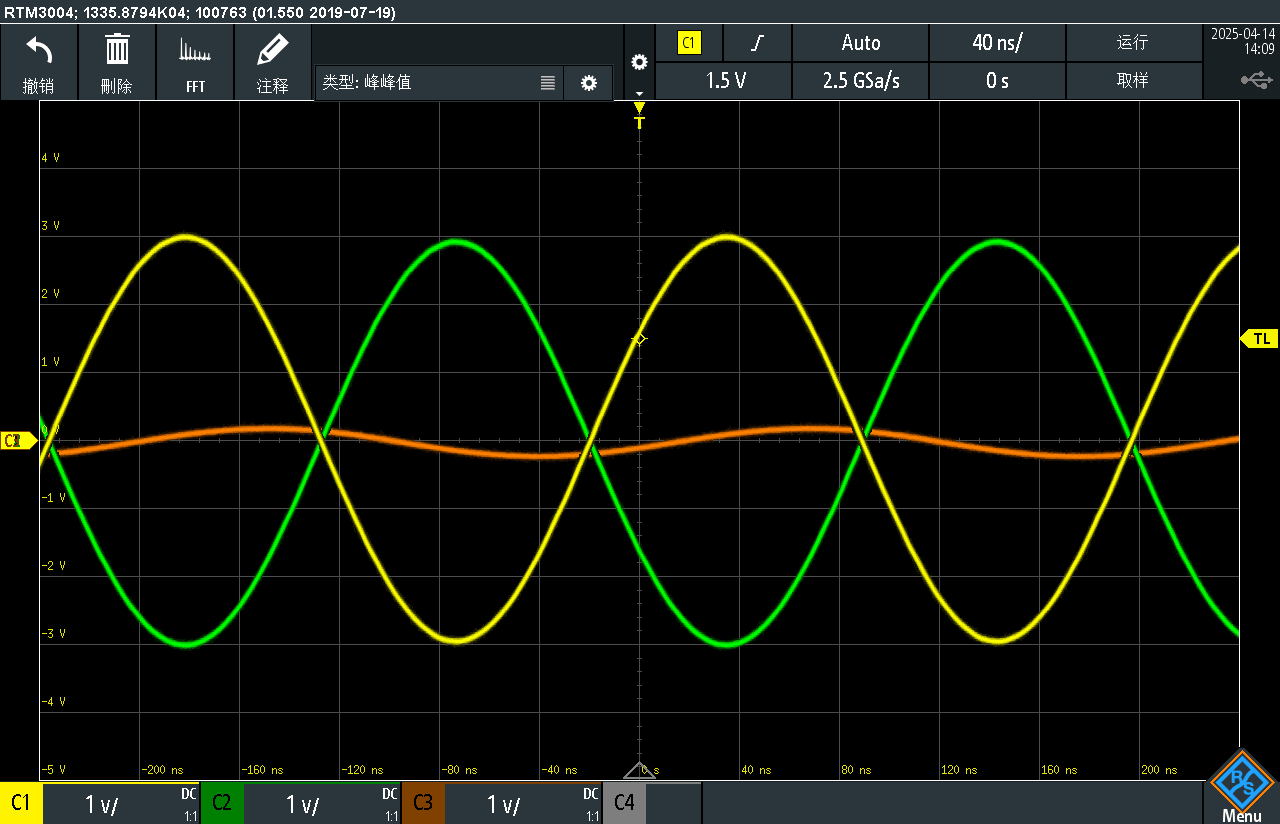
\includegraphics[width=0.8\textwidth]{SCR08.PNG}
    \caption{驻波状态下的同轴电缆信号 - 最低频}
    \label{fig:standing_wave_1}
\end{figure}

\begin{figure}[H]
    \centering
    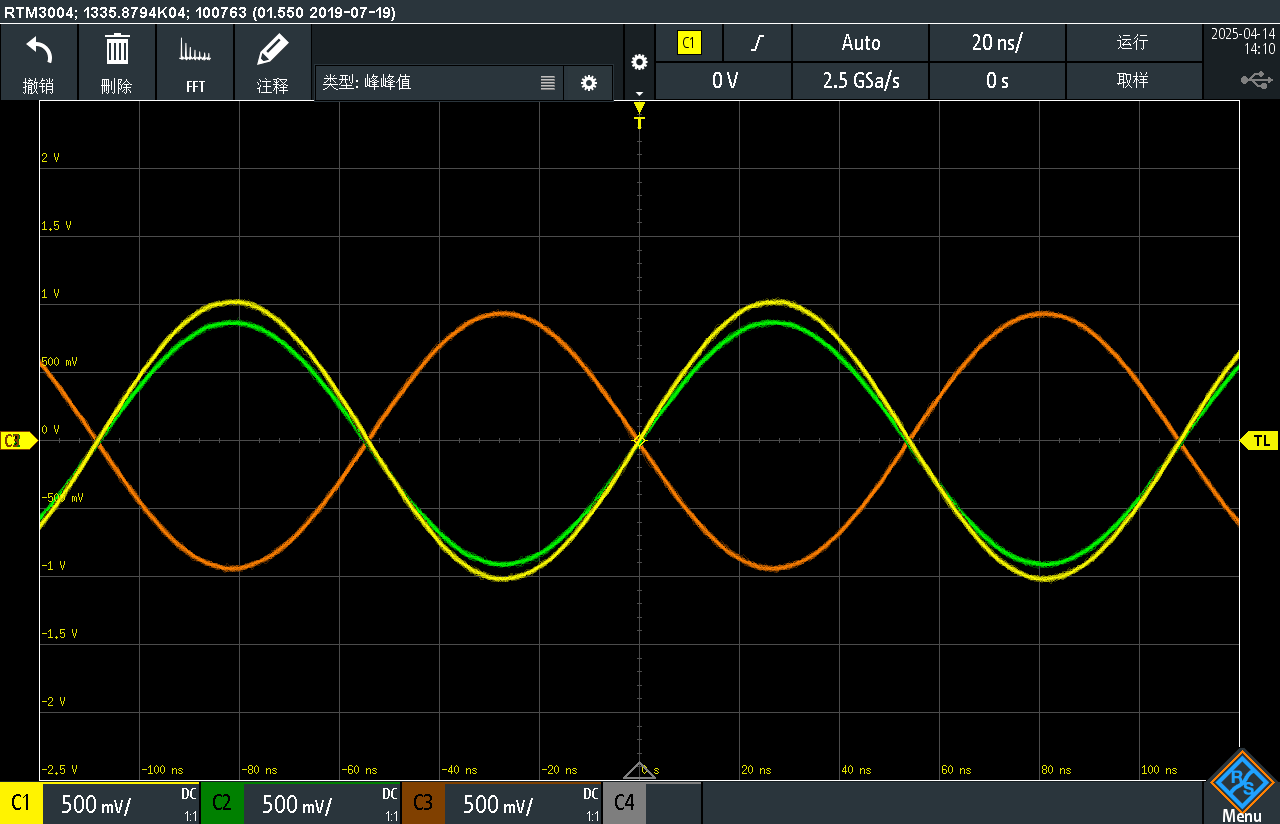
\includegraphics[width=0.8\textwidth]{SCR09.PNG}
    \caption{驻波状态下的同轴电缆信号 - 第 2 频}
    \label{fig:standing_wave_2}
\end{figure}

\definecolor{yellowwave}{HTML}{ecec00}
\definecolor{orangewave}{HTML}{dc6e00}
\definecolor{greenwave}{HTML}{00ea00}

其中,\textcolor{yellowwave}{黄色} 是入射处的电压波形,\textcolor{orangewave}{棕色} 是电缆中点处的电压波形,\textcolor{greenwave}{绿色} 是末端反射处的电压波形.

\section{分析与讨论}

思考题:假设实验中测试的同轴电缆为半无限长且无损耗 ($R=G=0$),其一端与信号发生器相连,另一端延伸到无穷远. 信号发生器设置为正弦波波形,电压峰峰值设为 $\SI{20}{\volt}_{pp}$、内阻为 $\SI{50}{\ohm}$,频率 $𝑓$ 为 $\SI{50}{\kilo\hertz}$. 问信号发生器对外输出功率吗?原因是什么?如果输出的话,功率是多大、存储在哪里?

这时候同轴电缆的特征阻抗为 $Z_0 = \sqrt{\frac{L}{C}}$,信号发生器的内阻为 $R_s = \SI{50}{\ohm}$,信号发生器的输出电压为 $V_s = \SI{20}{\volt}_{pp}$. 但是仍然有功率损耗,因为同轴电缆还是存在不为零的复阻抗. 信号发生器对外输出功率为:

\begin{equation}
    P = \frac{V_s^2}{Z_0 + R_s} = \SI{3.985}{\watt}
\end{equation}

输出的频率在空间中以电磁波的形式传播.

\section{原始数据截图}

\begin{figure}[H]
    \centering
    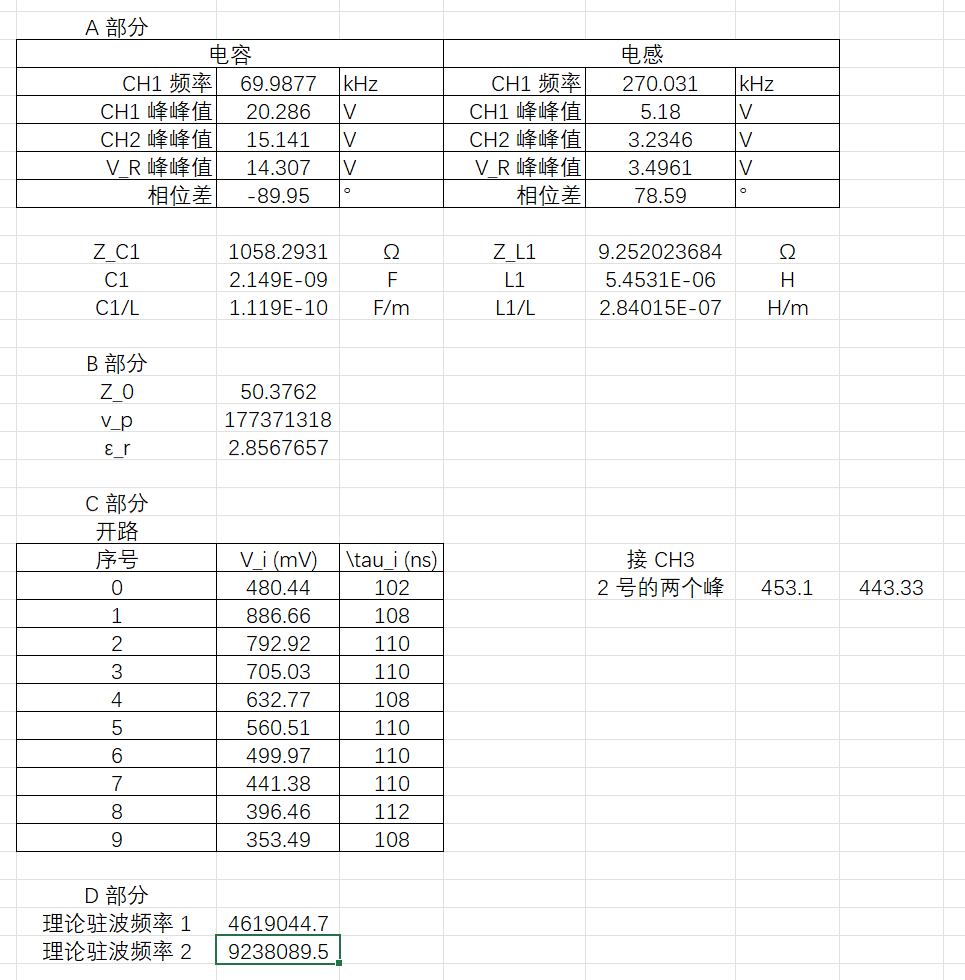
\includegraphics[width=0.8\textwidth]{originData.png}
    \caption{原始数据截图}
    \label{fig:original_data}
\end{figure}
\end{document}